\chapter{Implementation} \label{chap:implementation}

% - Image Reconstruction
% 	- Reconstruction algorithm (E2VID and data pre-processing etc.)
% 	- Computer vision techniques and models
% 		- NMNIST Classification
% 		- DVS128 Gesture Classification

% - Direct Event Classification
% 	- Data pre-processing etc. (talk briefly about working directly with events with nlp-like method)
% 	- Various model architectures
% 		- NMNIST Classification
% 		- DVS128 Gesture Classification

% - Converting previous networks to SNNs

\section{Video Reconstruction}

The models described above allow for the system to learn directly on the spiking data. Another approach that was taken was to attempt to utilise video reconstruction networks to the event data so that more classical models and architectures could be used to patterns in the data. It was interesting to note the performance differences between the previous networks and the described two-phase network.

\subsection{Reconstruction Algorithms}

\subsubsection{E2VID}

E2VID, as described in \color{red} TODO: Reference background reading here \color{black}, is a state-of the art network based on UNET that reconstructs intensity videos from events data. Having gotten the output from the network (which on test data had 90\% accuracy \color{red} TODO: check accuracy figure \color{black})

\color{red} TODO: all of the following;

\begin{itemize}
    \item Similar to denoising network CNN more easily able to find patterns in data
    \item gesture intensity maps equivalent to 100fps but retains high frequency information without too much noise
    \item spikingjelly for integrating frames which is widely used approach
\end{itemize}

\color{black}

\subsection{Classification Models on Reconstructed Video Output}

\section{Direct Classification of Events}

\subsection{Data Preprocessing}

\color{red} TODO: Add stuff about possible nlp-like networks. \color{black}

\subsubsection{Time-relative Event Segmentation}
In order to begin analysing neuromorphic data, it was pre-processed it into a form that a NN can take as input. One such method of doing so was to segment the events into groups based on their timestamp. \autoref{fig:nmnist_spikes_to_intensity_map} shows a visualisation of intensity maps created from the NMNIST\cite{NMNIST} dataset. The set of all events was split into eight segments, where each segment included events within a range of $ 1 \times 10^6 $ ms (i.e., $ 0 \rightarrow 1 $, $ 1 \rightarrow 2 $, ..., $ 7 \rightarrow 8 $). This way the data representation shifted to somewhat get back to a set of frames that mimicked the video output usually seen from everyday cameras. \textbf{(a)} shows the segmented events visualised in three dimensions (x\_location, y\_location and timestamp). In \textbf{(b)} these events were projected onto the two dimensional plane (of x\_location and y\_location), then the plots for on events and off events are shown separately. Finally in \textbf{(c)} an intensity map was created from the projected events. Each pixel in the intensity map grid was initialised to 0, and for every on event 1 was added to the cell, and for every off event 1 was subtracted from the cell. It was clear that the resulting output greatly resembled the MNIST\cite{MNIST} sample recorded by the ATIS camera (As shown in \autoref{fig:nmnist_spikes_visualisation} in \Cref{sec:existing_datasets}).

\begin{figure}[htb]%
    \centering
    \subfloat[\centering]{{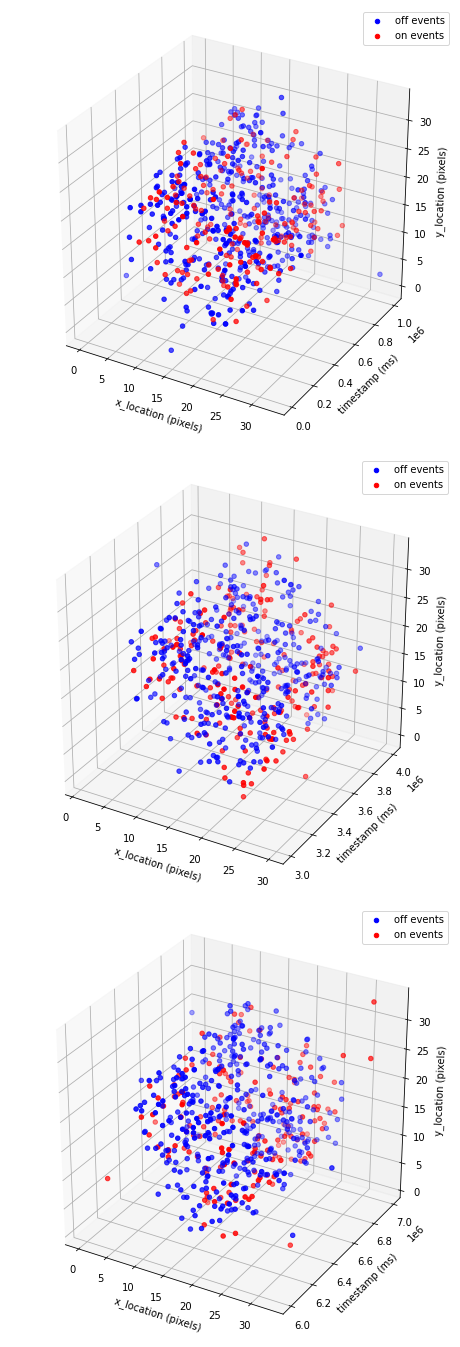
\includegraphics[width=0.25\textwidth, height=0.7\textwidth]{implementation/images/nmnist_spikes_visualisation_segmented.png}}}%
    \qquad
    \subfloat[\centering]{{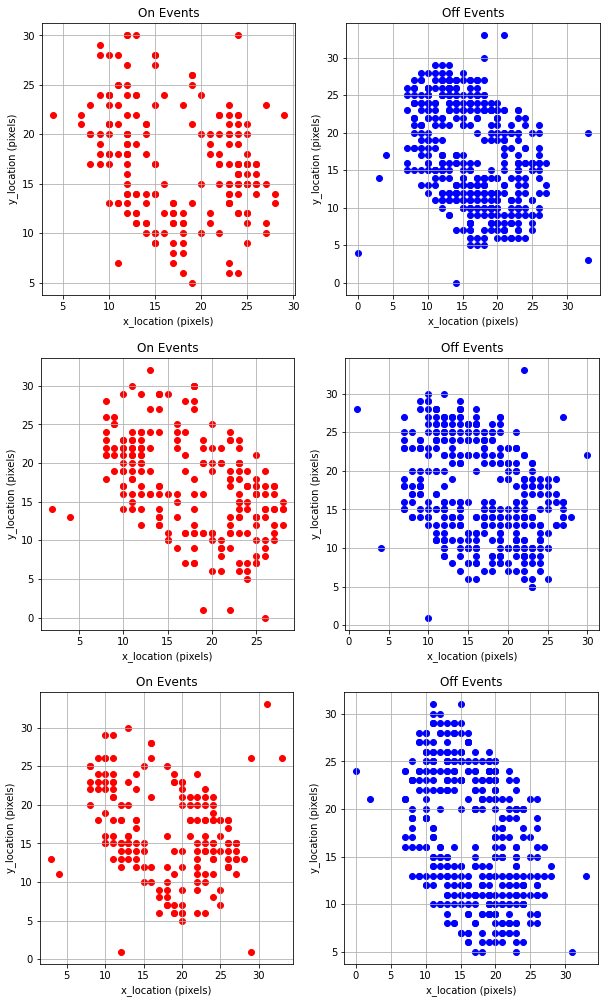
\includegraphics[width=0.4\textwidth, height=0.7\textwidth]{implementation/images/nmnist_events_segmented.png}}}%
    \qquad
    \subfloat[\centering]{{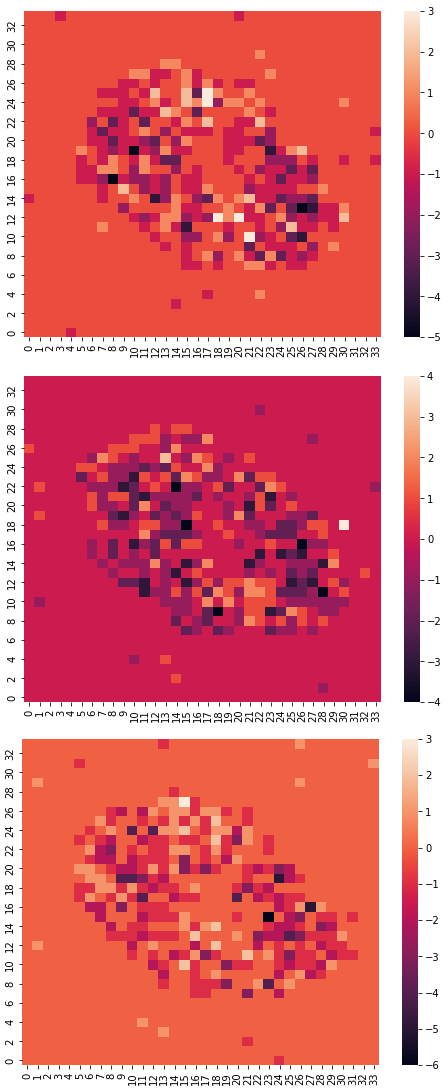
\includegraphics[width=0.25\textwidth, height=0.7\textwidth]{implementation/images/nmnist_events_heatmap_segmented.png}}}%
    \caption{A visualisation of intensity maps created by segmenting events into bins of size $ 1 \times 10^6 $ ms.}%
    \label{fig:nmnist_spikes_to_intensity_map}%
\end{figure}

Once a set of projections was made for each sample from the NMNIST dataset, it could be fed into a neural network in parallel. Ths could be done by simply flattening each intensity map and feeding all the cell values to a fully-connected dense layer in parallel, or the maps could be fed in as images to a convolutional layer. For the convolutional layer method a 3D tensor could be generated by stacking each of the intensity maps against each other and feeding them all directly into the first layer of the NN.

\subsubsection{Neural Network Input Structure}

There were many ways with which a neural network could accept an input to the system. The ones considered for this project where;

\begin{itemize}
    \item Flattening all the intensity maps from segmented event stream into a vector to be input to a single layer of neurons.
    \item Passing a 3D tensor to an convolutional layer as input.
\end{itemize}

\subsection{Classification Models}

\subsubsection{Pure Convolution Network}

Convolutional neural networks have been shown to be much more effective when processing images that networks built solely with dense, fully-connected layers \color{red} TODO: add references here \color{black}. This is because they are able to better identify spacial patterns within an image as a kernel spans more than one pixel. For this reason the basic architecture was to have an input layer (the structure of which is dependent on the input format), followed by a series of hidden convolutional layers of varying parameters.
However, since the input to the system is in fact a 3D tensor of multiple images (i.e. the intensity map video generated from the camera events) a typical convolutional network would not be sufficient to capture the temporal patterns in the data. Typically 2D convolution layers can take as input images with three channels (usually RGB), and so feasibly this coudld be extended to more channels for each frame of the video, but this is not a scalable approach. Instead 3D convolutional layers were used \cite{3DConv}.
Finally the outputs of the hidden layer were fed into a dense layer with 10 neurons to correctly classify the correct class (0-9). Activation functions need to be present in the network to prevent all the layers from becoming equivalent to a single one \color{red} TODO: add references here \color{black} (linear regression model). In order to learn more complex patterns activation functions are a necessary aspect of creating an artificial neuron (See \autoref{eq:artificial_neuron_output} in \Cref{ssec:snn_and_heterogeneity}). The most commonly used activation function in deep networks (and image recognition in particular), and in this network as well, is ReLU. \color{red} TODO: add references here \color{black}. Finally, the output layer has a sigmoid activation function. This function compresses the output smoothly between the ranges of 0 and 1. this means each of the outputs from the neurons can be interpreted as a the probability of the input being any one of the 10 classes. This means we can simply take the highest probability as the predicted class from the network.

Hyper-parameter Tuning:

In order to choose the most appropriate parameters for the system, multiple tests were run varying each of the possible hyper-parameters. The tests conducted were to determine;

\begin{itemize}
    \item The number of hidden layers.
    \item The number of neurons per layer.
    \item The size of convolution kernels.
    \item The introduction of some fully connected layers after convolutional layers.
\end{itemize}

The network in each case was trained for multiple epochs. The performance of a typical network can be seen in \autoref{fig:accuracy_and_loss_per_epoch}, where the performance on the training set steadily improves as the network progresses through epochs. Accuracy is one of the metrics defined in \cref{sec:evalutaion_metrics}, and the loss for the given network is called categorical cross-entropy loss. The formula used to calculate the loss is given by: $ L = -\frac{1}{N}\sum^N_{i=1}\sum^C_{c=1}y_c^{(i)}log(\hat{y}_c^{(i)}) $, where there are $ N $ samples and $ C $ classes. $ y_c^{(i)} $ is $ 1 $ when the class is correctly predicted and $ 0 $ otherwise and $ \hat{y}_c^{(i)} $ is the predicted probability of class $ c $ for data-point $ i $.

\begin{figure}[htb]
    \centering
    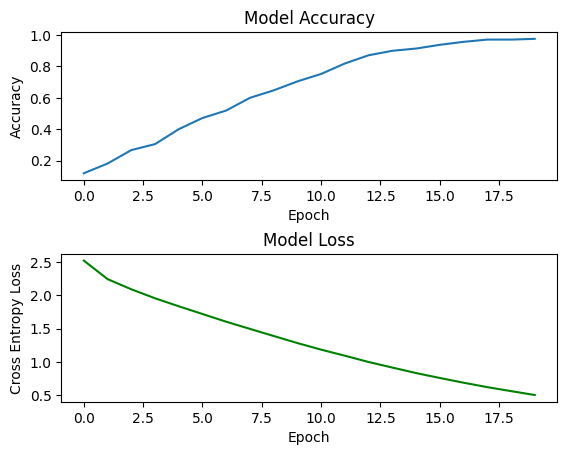
\includegraphics[width=0.4\textwidth]{implementation/images/accuracy_and_loss_per_epoch.png}
    \caption{A figure showing classification accuracy and cross-entropy loss per epoch on training data for a typical network.}
    \label{fig:accuracy_and_loss_per_epoch}
\end{figure}

It was clear, however, that these results may be misleading since they only represent the efficiency of the system when classifying values within the training data-set. However, when looking at the performance on an unseen test data-set, it is obvious that some of the features learnt do not easily translate to general trends in unseen data. This is known as over-fitting, and can be avoided by reducing the capacity of the data-set so that it does not learn information specific to the training set.

Model capacity is directly correlated to the n$ ^o $ of filters, as well as the number of layers, and as the model recognises more patterns in the training data, so it is important to get the optimum value for the system. The size of the kernels has an effect on the scale of the information picked up by the system. With smaller kernels more local patterns are detected, whereas with larger kernels more global effects can be seen \color{red} TODO: add image and reference here \color{black}. As for the dense layers at the end of the network, it can be seen that better results were achieved as a result of it since global patterns can be further identified after the data has been processed by the convolution layers that have picked out the most important features.

\begin{figure}[htb]%
    \centering
    \subfloat[\centering]{{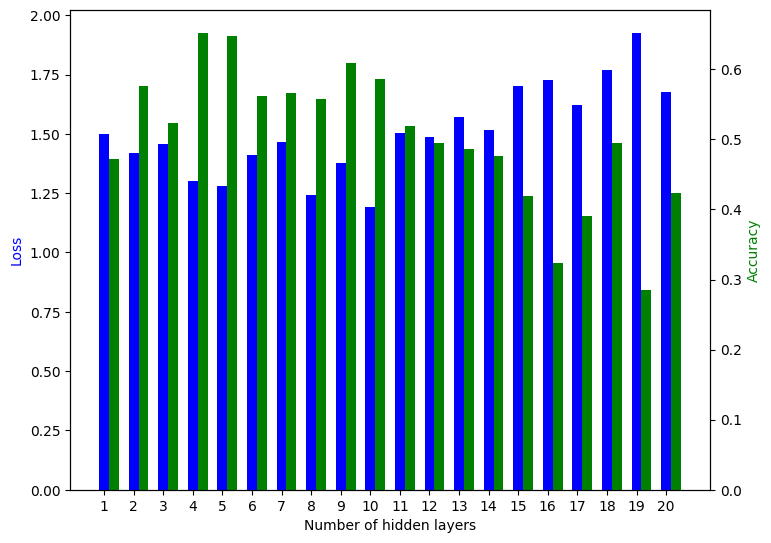
\includegraphics[width=0.4\textwidth]{implementation/images/layer_tests.png}}}%
    \subfloat[\centering]{{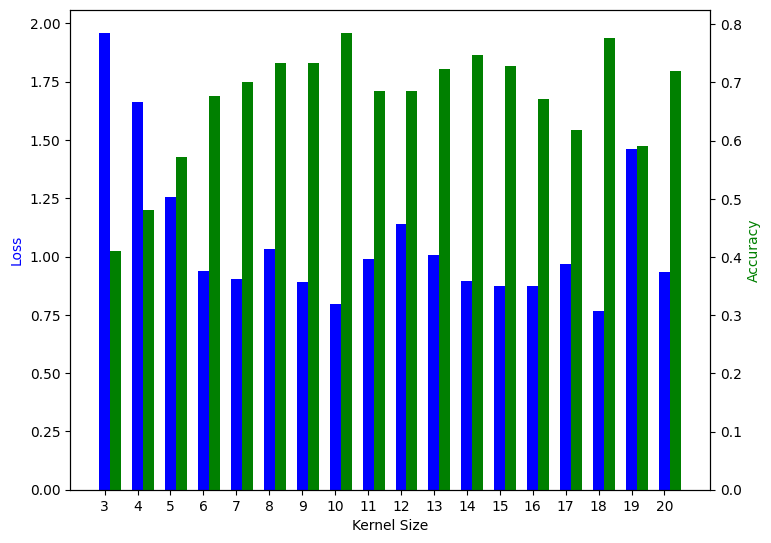
\includegraphics[width=0.4\textwidth]{implementation/images/kernel_tests.png}}}%
    \hfill
    \subfloat[\centering]{{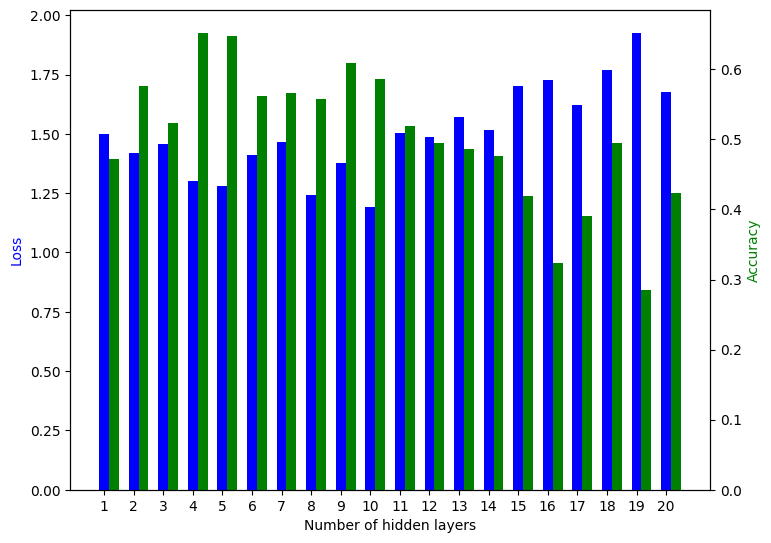
\includegraphics[width=0.4\textwidth]{implementation/images/layer_tests.png}}}%
    \subfloat[\centering]{{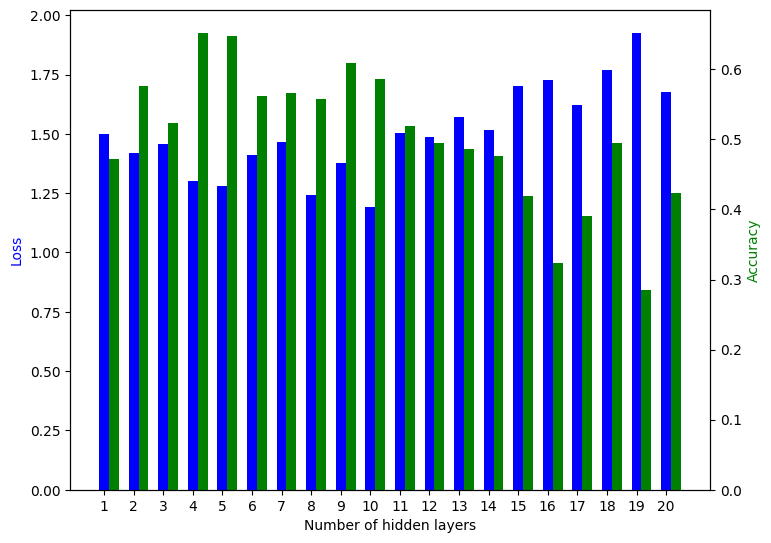
\includegraphics[width=0.4\textwidth]{implementation/images/layer_tests.png}}}%
    \caption{A visualisation of intensity maps created by segmenting events into bins of size $ 1 \times 10^6 $ ms.}%
    \label{fig:tests}%
\end{figure}

Further testing was done with increasing kernel sizes, and with pooling layers added to the network. To find local patters filter kernels smaller than the image (32x32) are used. In earlier layers the no of filters is
large and the filter size is small to capture details. The no
of filters decreases and the filter size increases later in the
network for higher-level patterns. Pooling filters the image
after convolution layers to pick out important features. \color{red} TODO: add final system architecture here \color {black}.

\subsubsection{LTSM}

\subsubsection{Convolutional LTSM}

LTSM networks show promise in their ability to find patterns not only on an frame-by-frame basis but also in the time dimension. These spatio-temporal patterns are much more effective for classifying image sequences that just spatial patterns since information is carried throughout the frames to find overall movements and gestures. These LTSMs utilise fully connected layers to find patterns in each frame, however it has been shown that convolutional neural networks produce much better results when operating on image data, and so it would stand to reason that LTSMs would benefit from their structure as well. ConvLTMS, developed by \textit{Xingjian SHI et al.}, showed great promise, and in their experiments captured spatio-temporal correlations better and more consistently FC-LSTM, outperforming it by a sizeable margin in the application of forecasting.

\color{red} TODO: Show model of custom Conv3D network \color{black}

\section{Spiking Neural Network}

\color{red} TODO: Cite nengo etc. \color{black}

\subsection{Synaptic Smoothing}

\subsection{Firing Rates}

\subsubsection{Post-training Scaling}

\subsubsection{Regularizing During Training}